\section{De-featuring using feature information}
	
	De-featuring involves removing small-irrelevant features like Holes, Fillets, Chamfers. Detection and suppression becomes relatively straightforward with the ready feature-information rather than doing similar process on just the Boundary Representation (Brep). Use of features such as Pattern, Mirror can also be leveraged to detect symmetry for keeping just the master portion for reduced analysis. 

\subsection{Literature Survey}

Dabke \citep{Dabke1994} through the concept of Global Idealization was one of the first ones to leverage use of feature information for de-featuring. 

	 Lee \citep{Lee2005} elaborated a method to reorder design features in the history tree and then to re-execute the history of the reordered features up to the given level of simplification. Since Brep re-evaluation is computationally intensive, he used cellular model for increasing the performance. Many of the commercial CAD models being Brep-CSG (Constructive Solid Geometry) based, converting to the cellular one would again be a time consuming step.

Approaches like that of Hamdi \citep{Hamdi2005}  seem to test individual features for removal, but approach in this paper takes into account the parent-child relationship between features as well. Russ \citep{Russ2012} had hinted about taking care of child features arising out of dependencies. 

	Modeling history may be different for similar final shape. So Model Simplification processes based on feature history tree could yield different results. To achieve consistent simplification results independent of the modeling history, some attempts use just the final Brep model, then recognize features to be removed directly from that final model.  But recognizing features is still not a very deterministic process. Woo \citep{Woo2009} proposed a new method which has subtractive features recognized directly from final solid thus eliminating problem of looking at the history tree. 

Even if there are few limitations as stated above, having ready feature information is far better than trying to recognize features in Brep or using decomposition methodologies to split Brep into simpler shapes.

\subsection{Proposed Approach}

In many CAD applications, model-history or the feature tree is readily available. This makes the task of de-featuring easier since their parameters can directly be used to qualify for suppression. The model feature tree is traversed and candidate features for suppression are identified based on a set of criteria. Suppression or removal of these features results in a much simplified model, suitable for creating meaningful Midsurface. 

Algorithm \ref{alg1} explains the process of de-featuring . Table \ref{DefeatRules} summarizes various rules used for qualification of a feature for suppression and Table \ref{DefeatTestcases} presents application of various rules and their effects. 


\begin{longtable}{L{0.45\textwidth}  L{0.55\textwidth}}
\caption{Suppression Qualifications}\\
\hline
{\bf Feature Type} & {\bf Dimension chosen for comparison against Part size threshold} \\
\hline
\hline
%------------------------------------------------------------------------------------------------------------------------------------
Hole &
Diameter (however long Height may be) \\


%------------------------------------------------------------------------------------------------------------------------------------
Fillet &
2*Radius (however long Length may be) \\


%------------------------------------------------------------------------------------------------------------------------------------
Chamfer &
Max Side (however long Length may be) \\


%------------------------------------------------------------------------------------------------------------------------------------
Primitives (+ve, -ve, standalone) &
(Self + Children ) Bounding Box diagonal \\

%------------------------------------------------------------------------------------------------------------------------------------
Sweep Based (+ve, -ve, standalone) &
(Self + Children ) Bounding Box diagonal\\


%------------------------------------------------------------------------------------------------------------------------------------
Mirror, Patterns &
Keep Master (No Size Criterion)\\
\hline

\label{DefeatRules}
\end{longtable}


Care should be taken while selecting features to suppress, as removal of certain features (e.g. fillets) will increase the stresses in a part, so that the results of the FEA analysis will be conservative. Features in the load path or near boundaries where boundary conditions are applied need to skipped from de-featuring.

\begin{algorithm}
	\caption{De-featuring by suppressing certain features}
	\label{alg1}
	\begin{algorithmic}
		\REQUIRE A CAD model with access to the feature tree
		\STATE {\bf Size criterion}: Get Part's Bounding Box ({\bf pBB}), it's diagonal length 
		\STATE Get a threshold (say, 5\%) to calcuate the threshold size = threshold x diagonal
		\STATE Calculate the threshold size {\bf D} below which a feature(set) is considered  'small'
		\STATE  Initialize Suppress feature list {\bf SL} to which features will get added
		\WHILE{End of tree has  not reached}
			\STATE Get the current feature.
			\STATE Get Bounding Box ({\bf fBB}) of the current feature 
			\STATE Find diagonal length d of the {\bf fBB}
			\IF {feature type is Hole}
				\STATE Add to {\bf SL} if Diameter  <   {\bf D}
			\ENDIF
			\IF {feature type is Tweak}
				\STATE  Fillet or Chamfer: Add to {\bf SL} if Radius or Side  <  {\bf D}
			\ENDIF
			\IF {feature type is Mirror or Pattern}
				\STATE  Keep Master (No Size Criterion)
			\ENDIF
			\IF {feature type is Sweep Based (Extrude, Revolve etc.) or Primitives (Block, Cylinder etc.), Protrusions or Depressions or Standalone}
				 \STATE Get all the child features and update the Bounding Box to ({\bf fcBB}) with the Union of Bounding boxes of self + child features (called feature-set {\bf FS}). 
				\STATE Find diagonal  {\bf d} of {\bf fcBB}. Add {\bf FS} to {\bf SL} if  {\bf d} <  {\bf D}
			\ENDIF
		\ENDWHILE
		\STATE  Regenerate model by excluding the features in {\bf SL}
		\STATE  Validate the model
	\end{algorithmic}
\end{algorithm}

\begin{longtable}{ | C{0.25\textwidth}  L{0.25\textwidth} || C{0.25\textwidth}  L{0.25\textwidth}|}
\caption{De-featuring rules and their effect}\\
\hline
{\bf Detection} & {\bf Explanation} & {\bf Detection} & {\bf Explanation}\\
\hline
\hline

%------------------------------------------------------------------------------------------------------------------------------------
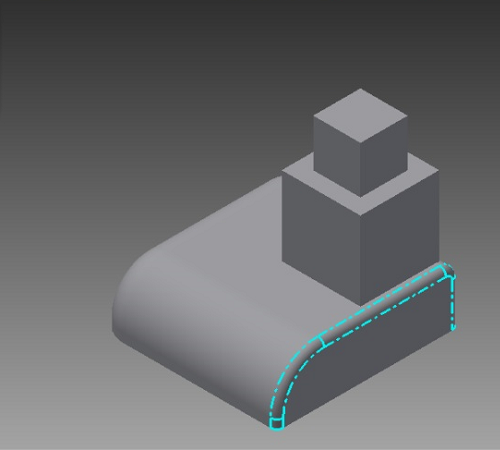
\includegraphics[scale=0.236]{..//Common/images//defeat1.png} &
At 5 \% threshold smaller fillets are detected. Rest of the part is shown to get idea of the parts size &
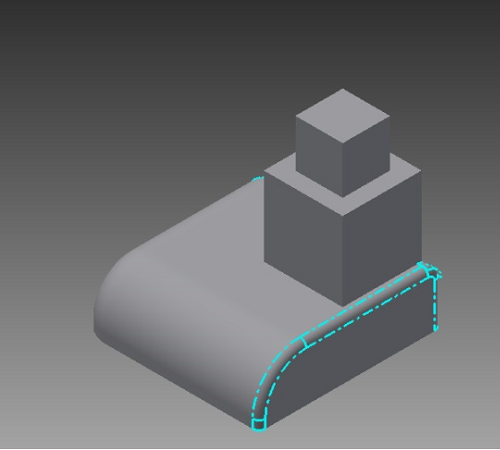
\includegraphics[scale=0.236]{..//Common/images//defeat2.png} &
More fillets detected at 10 \% threshold\\


%------------------------------------------------------------------------------------------------------------------------------------
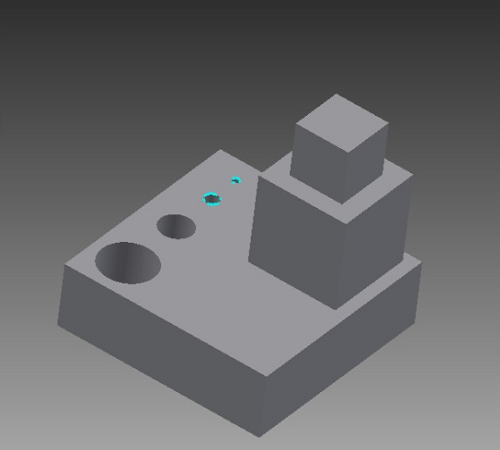
\includegraphics[scale=0.236]{..//Common/images//defeat3.png} &
Smaller holes detected at 5 \% threshold &
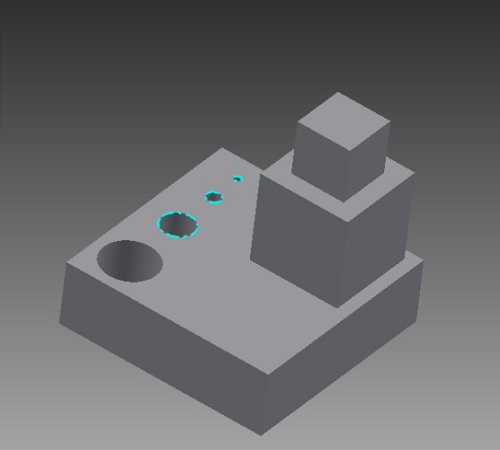
\includegraphics[scale=0.236]{..//Common/images//defeat4.png} &
More holes are detected at 10\%  threshold\\


%------------------------------------------------------------------------------------------------------------------------------------
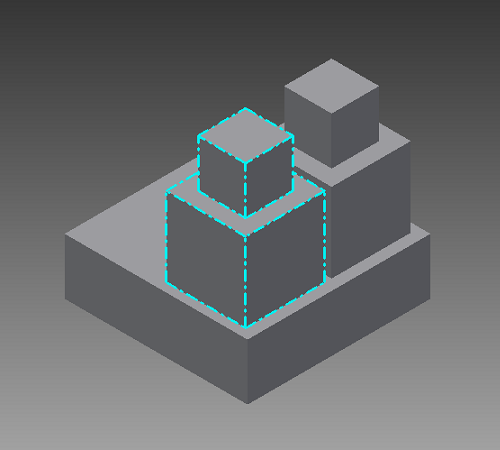
\includegraphics[scale=0.236]{..//Common/images//defeat5.png} &
Even if individually each feature is big enough when they are Mirrored they qualify for suppression &
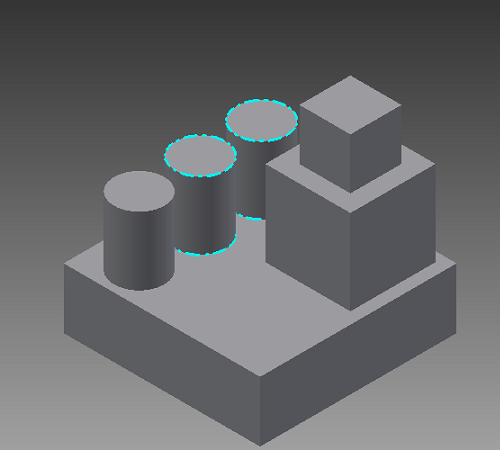
\includegraphics[scale=0.236]{..//Common/images//defeat6.png} &
Even if individually each feature is big enough when they are Patterned they qualify for suppression \\


%------------------------------------------------------------------------------------------------------------------------------------
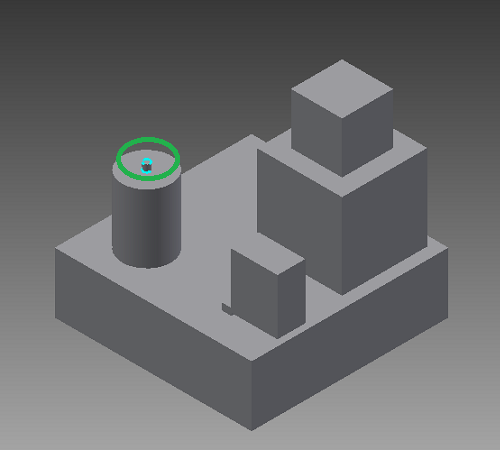
\includegraphics[scale=0.236]{..//Common/images//defeat7.png} &
Smaller cylindrical Extrusion got detected. It’s a child of Bigger cylinder.  & 
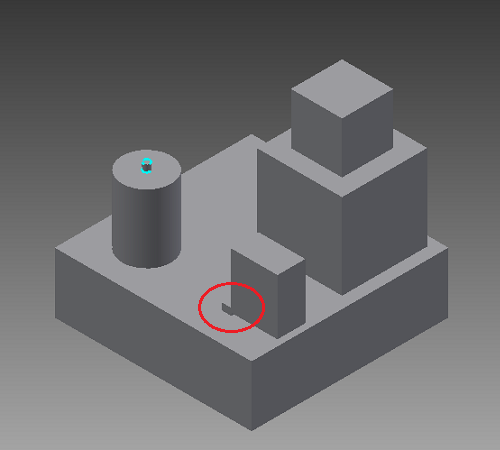
\includegraphics[scale=0.236]{..//Common/images//defeat8.png} & 
But small rectangular extrusion did not get selected as its child (bigger block) has disqualified him\\
\hline

\label{DefeatTestcases}
\end{longtable}

%=================================================================================================================

\subsection{Examples}

For validation of the approach a part with medium complexity is run through the Algorithm \ref{alg1} to evaluate its correctness.

\begin{longtable}{ C{0.28\textwidth}  C{0.28\textwidth}  L{0.4\textwidth}}
\caption{Sample Cases}\\
\hline
{\bf Preview} & {\bf Results} & {\bf Comments} \\
\hline

%------------------------------------------------------------------------------------------------------------------------------------
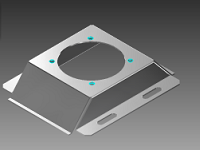
\includegraphics[scale=.72]{..//Common/images//defeatmodel1.png} &
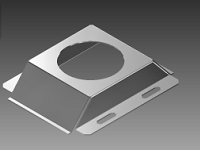
\includegraphics[scale=.72]{..//Common/images//defeatresult1.png} &
Holes in Circular Pattern are detected and have been suppressed as shown in 'Results'\\


%------------------------------------------------------------------------------------------------------------------------------------
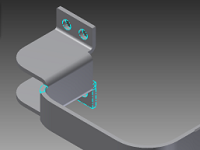
\includegraphics[scale=.72]{..//Common/images//defeatmodel2.png} &
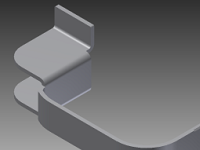
\includegraphics[scale=.72]{..//Common/images//defeatresult2.png} &
Small Holes in Mirror are detected. Large fillets are not detected as their sizes are more than the threshold. \\


%------------------------------------------------------------------------------------------------------------------------------------
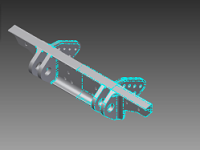
\includegraphics[scale=.72]{..//Common/images//defeatmodel3.png} &
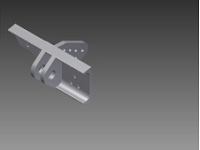
\includegraphics[scale=.72]{..//Common/images//defeatresult3.png} &
Mirror is detected, by suppression of which half part remained. Most of the holes are not detected as they are not small enough. \\
\hline
\label{Defeat}
\end{longtable}


The de-featured model can then be taken for meshing or can be used for Midsurface generation.

%=================================================================================================================

\section{Idealization using feature information}

In Idealization, slender potions are abstracted to lines-curves where as for the thin plate-like portions Midsurface is used as an idealized form.  This paper focuses on Midsurface generation aspect of the idealization.
%	\begin{figure}
%	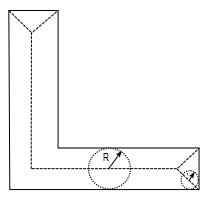
\includegraphics[scale=0.5]{..//Common/images//MAT.png}
%	\caption{Medial Axis Transform}
%	\label{MAT}
%	\end{figure}
%	
	
	\begin{wrapfigure}{l}{0.4\textwidth}
	\centering
	\vspace{-.6cm}
	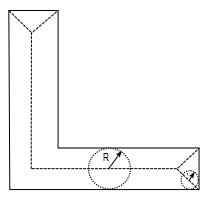
\includegraphics[scale=0.65]{..//Common/images//MAT.png}
	\vspace{.2cm}
	\caption{Medial Axis Transform}
	\label{MAT}
	\vspace{-.5cm}
	\end{wrapfigure}

Such idealized shapes need to connect with neighbors keeping no gaps and following shape of the parent part. In Mid-surfacing techniques there are two broad categories namely, 'Medial Axis Transform (MAT)'   (Figure \ref{MAT}) and 'Midsurface Abstraction(MA)'   (Figure \ref{Abstraction}). 

MAT is  loci of the centers of an inscribed disc of maximal diameter as it rolls around the object interior.  In 2D its called Medial Axis Curve and in 3D it is called as Medial Surface. As evident in the Figure  (Figure \ref{MAT}) major problem of this method is that it creates unnecessary branches and the medial shape is smaller than the original corresponding contour. 

MA (Figure \ref{Abstraction}) involves finding  'pairs of surfaces', constructing 3D mid-surface between them and then sewing the mid-surface patches to make a continuous idealized surface. This surface-pairing approach has benefits over MAT techniques because the resultant geometry is cleaner and requires less reconstruction. However the surface pairing approach is challenging as it can be difficult to identify all of the surface pairs.

\subsection{Literature Survey}

One of the early works in the field of medial entity was by Harry Blum in 1967 \citep{Harry1967}. Survey papers like \citep{Attali2004}, \citep{Lam1992} and \citep{Yogesh2010, YogeshCOEP2013} have detailed various approaches used so far. 


Ramanathan \citep{Ramanathan2004} enhanced MAT method to remove erroneous branches to a certain extent, typically for the simple shapes. As many of the MAT algorithms are piecewise polygonal approximations, Fischer \citep{Elber1999} suggested method of parametric mid-curves which would have no branches and would represent shape of the parent curves. In this method finding edge-face pairs in the shape is a non-trivial task. 

%	\begin{figure}
%	\includegraphics[scale=0.5]{..//Common/images//Midsurface.png}
%	\caption{Midsurface Abstraction Methods}
%	\label{Abstraction}
%	\end{figure}
	
	
	\begin{wrapfigure}{l}{0.6\textwidth}
	\centering
	\includegraphics[scale=0.4]{..//Common/images//Midsurface.png}
	\caption{Midsurface Abstraction Methods}
	\label{Abstraction}
	\vspace{-1cm}
	\end{wrapfigure}



Hamdi et.al. \citep{Hamdi2005} used feature information for removal of small details and also while idealizing basic primitives like Parallelepipeds, Cylinder and Wedge. 

Robinson et. al.  \citep{Robinson2006} utilized CAD feature tree to locate sketches. Slender regions in the sketch were used to create sheet bodies representing thin regions of the component. He based detection and medial creation on the MAT method. 

Roland Stolt \citep{Stolt2005, Sunnersjo2005, Stolt2006} developed feature based Midsurface for features like Pad and Pocket. He  elaborated on treatment of negative volumes, fillets but not much on mid-curves for complex 2D profiles. Also, his work had restrictions like of using thin wall parts with constant thickness and did not provide thickness values on the Midsurface which is necessary for creating Shell elements. 

Sheen  \citep{Sheen2008} mentioned that due to complexity in recognizing forms, and due to complex interactions between them, typically, Midsurface of the part does not follow form of the base part and is not fully connected . 

Smit \citep{Smit2011} linked CAD and CAE model through individual features. A method was developed to qualify features for abstraction but connecting them together became a challenging task. These techniques, in primitive ways, have used feature information to create idealization for individual features but he did not elaborate much on how feature interactions are dealt with.

Recently, Woo \citep{Woo2013} proposed a method to decompose a  shape into smaller manageable primitives, for which Midsurface can be generated. His work has presented very simple cases, with not much elaboration on how extend-trim-joining of individual patches, will work in non-trivial cases. Main limitation of his approach is that quality of Midsurface depends on the success of the decomposition as well as how interactions between primitives are handled.

This paper proposes a solution of creating Midsurface as the CAD model is getting built.


%===============================================================================

\subsection{Proposed Approach}

In Feature-based Solid Modeling, for construction features,  input parameters are used to build tool-bodies. These tool bodies are then boolean-ed with the base part. In many cases the tool-bodies are relatively simple shape. In the proposed approach  (as listed in Algorithm \ref{alg2}), Midsurface is generated for the tool-bodies, at an individual feature level. With the boolean between the base part (which already has Midsurface built in) and tool-bodies, their respective Midsurfaces are boolean-ed as well thus resulting in well connected, isomorphic Midsurface. 

\begin{algorithm}

	\caption{Midsurface creation on per feature basis }

	\label{alg2}

	\begin{algorithmic}

		\REQUIRE A CAD model (preferably de-featured) with access to the feature tree

		\WHILE{End of tree has  not reached}

			\STATE Get the current feature.

			\IF {feature type is Sketch}
				\STATE  If information regarding Sketch sub-commands like 'Sketch-Offset', 'Circle', 'Rectangle', are available, they can be leveraged to create standard mid-curves. 
				\STATE If such information is not available, slender portions need to be identified using MAT and then post-processed MAT curves can be used as mid-curves.
			\ENDIF

			\IF {feature type is Primitives}
				\STATE  For positive primitive shapes (protrusions or stand-alones) create a predefined Midsurface
			\ENDIF

			\IF {feature type is  Sweep based Features (Extrude Sweep Revolve Loft)}
				\STATE For positive primitive shapes (protrusions or stand-alones) sweep Mid-Curves profile similar that of the parent feature.
			\ENDIF

			\IF {feature type is Boolean (External)}
				\STATE Extend and Trim the Midsurface coming from Base part and Tool bodies.
			\ENDIF

			\IF {feature type is Tweak}
				\STATE Features like Fillet, Chamfer, ignore if small as part of the de-featuring process.
			\ENDIF

			\IF {feature type is Shell}
				\STATE  Use half the Shell distance and offset the same faces as in the parent feature to arrive at the Midsurface.
			\ENDIF

			\STATE Intersect Midsurface with the feature faces to make sure that it lies inside the feature volume.

			\STATE Assign the Thickness values on the Midsurface with predefined grid spacing.

		\ENDWHILE
		\STATE Midsurface gets built as part gets developed feature by feature.
		\STATE Check for validity of the Midsurface output, especially for gaps and overlapping surfaces and correct the problems

	\end{algorithmic}

\end{algorithm}


In traditional MA approach, detecting face pairs is a challenge. Even for simple shapes having connections like ’T’, 'Y', ’X,’ one needs to formulate rules for grouping face-pairs based on adjacency so that common connections get created. In more complex situations, it becomes more difficult to get Midsurface from individual sub-shapes to get connected at the common junctions. In the proposed approach where you start creating Midsurface as part is being built, at-least one operand in the boolean, called tool bodies, is typically simpler. As the interaction-boolean type is known it can be leveraged to arrive at well-connected Midsurface. 

The procedure of creating Midsurface in the existing MA approach and in the newly proposed approach would be different also. For example, in case of, say, simple plate, the existing approach would find face pairs, get their individual surface geometries, get sample points and create mid-offset surface between the paired faces. In the proposed approach, the plate would correspond to an Extrude feature. The feature would have elongated rectangle as a sketch-profile which then gets extruded by some distance in the normal direction. Here the mid-curve (a line) is created in the sketch profile itself. This mid-curve will get extruded similarly along with rest of the profile thus mimicking shape well. This tool body when will join by extend-trim to the base part. In case where the whole rectangle is extruded in the thickness direction, again no face pair needs to be detected. One has to just offset the base face by half the thickness.


%=================================================================================================================
\subsection{Example}

A part with medium complexity is run through the algorithm to evaluate its validity.

%\begin{table}[!h] % longtable does not work inside Table block
%\vspace{-2cm}

%\onecolumn % long table does not work in two-column mode

\begin{longtable}{ L{0.18\textwidth} C{0.18\textwidth} L{0.38\textwidth}  C{0.18\textwidth}}
\caption{Step by step creation of part along with Midsurface}\\
\hline
{\bf Modeling Input} & {\bf Modeling output} & {\bf Procedure to create Midsurface} & {\bf Midsurface}\endhead
\hline
\hline
%------------------------------------------------------------------------------------------------------------------------------------
Sketch Feature:
Create Rectangle (Length, Width) &
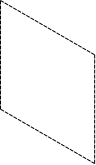
\includegraphics[scale=0.3]{..//Common/images//DryRun1.png} &
For non-thin profile like this, no mid-curve entities are created. For thin profiles, they are created. &
- \\
\hline
%-------------------------------------------------------------------------------------------------------------------------------------- 
Sketch Feature: Add Circle as inner loop &
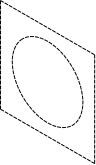
\includegraphics[scale=0.3]{..//Common/images//DryRun2.png} &
For non-thin profile like this, no mid-curves are created. If inner geometry was rectangle making concentric profiles, mid-curves would be generated. &
- \\
\hline
%-------------------------------------------------------------------------------------------------------------------------------------- 
Offset/Face/Thicken Feature: Thickness &
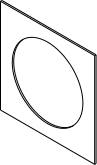
\includegraphics[scale=0.3]{..//Common/images//DryRun3.png} &
Fill the face with sketch curves and Offset it by 0.5*thickness value. In case of mid-curves in sketch, just extrude by 0.5*thickness value. &
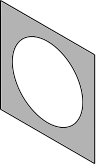
\includegraphics[scale=0.3]{..//Common/images//DryRun31.png} \\
\hline
%-------------------------------------------------------------------------------------------------------------------------------------- 
Flange (Edge, distance, angle)  &
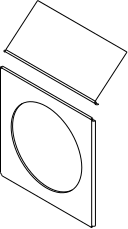
\includegraphics[scale=0.3]{..//Common/images//DryRun4.png} &
For Flange tool body, create Midsurface with given parameters. Need to find out corresponding edge on previously created Midsurface, to attach this tool-Midsurface to. &
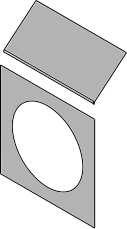
\includegraphics[scale=0.3]{..//Common/images//DryRun41.png} \\
\hline
%-------------------------------------------------------------------------------------------------------------------------------------- 
Similarly add other Flanges  &
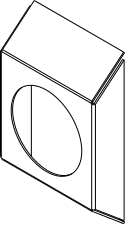
\includegraphics[scale=0.23]{..//Common/images//DryRun5.png} &
Similarly join other tool-Mid-surfaces &
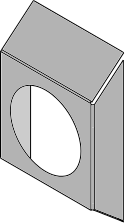
\includegraphics[scale=0.23]{..//Common/images//DryRun51.png} \\
\hline
%-------------------------------------------------------------------------------------------------------------------------------------- 
Ready Extensions, or user defined features booleaned  &
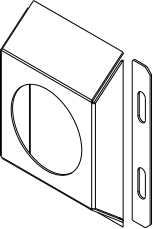
\includegraphics[scale=0.23]{..//Common/images//DryRun6.png} &
Tool bodies need to follow same Midsurface procedure and then Boolean them. Here complexities like L, T, K shapes come into picture. Need to come up with various heuristics for such connections.  &
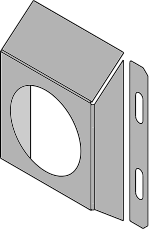
\includegraphics[scale=0.25]{..//Common/images//DryRun61.png} \\
\hline
%-------------------------------------------------------------------------------------------------------------------------------------- 
Similarly add other Flanges  &
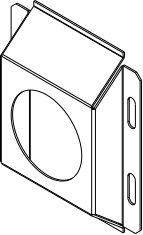
\includegraphics[scale=0.23]{..//Common/images//DryRun7.png} &
Similarly join other tool-Mid-surfaces &
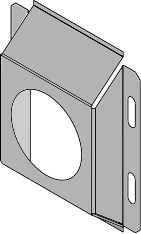
\includegraphics[scale=0.23]{..//Common/images//DryRun71.png} \\
\hline
%-------------------------------------------------------------------------------------------------------------------------------------- 
Add small holes &
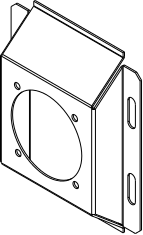
\includegraphics[scale=0.23]{..//Common/images//DryRun8.png} &
No change in Midsurface as small holes are ignorable. This takes care of Model Simplification as well. &
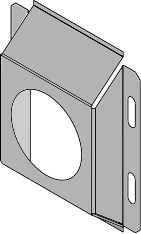
\includegraphics[scale=0.23]{..//Common/images//DryRun81.png} \\
\hline
%-------------------------------------------------------------------------------------------------------------------------------------- 
\label{DryRun}

\end{longtable}

%\twocolumn % long table does not work in two-column mode, resetting back

%\end{table}
This method has vast scope of further development due to large number of feature types,in domains not restricted to Solid Modeling domain but also in the environments like Sheet Metal Modeling, Injection Molding etc.

